\documentclass[a4paper]{article}

\usepackage{amsmath}
\usepackage{amsfonts}
\usepackage{anysize}
\usepackage{enumerate}
\usepackage{float}
\usepackage{graphicx}
\usepackage{hyperref}
\usepackage{listings}
\usepackage{SIunits}

\marginsize{2.5cm}{2.5cm}{1.5cm}{1.5cm}
\setlength{\parindent}{0pt}

\graphicspath{{./images/}}

\title{Design of Digital Platforms}
\author{Pieter Maene}
\date{\today}

\begin{document}
\lstset{
    language=C,
    numbers=left,
    stepnumber=1,
    numbersep=10pt,
    backgroundcolor=\color{white},
    showspaces=false,
    showstringspaces=false,
    showtabs=false,
    tabsize=2,
    captionpos=b,
    breaklines=true,
    xleftmargin=30pt,
    basicstyle=\ttfamily, 
    breakatwhitespace=true
}

\maketitle

\section{Analysis of Previous Design}

The design we built for the winter evaluation had the performance metrics listed in Table~\ref{tab:performance_metrics_winter} and the synthesis results from Table~\ref{tab:synthesis_results_winter}. Four shared memory locations (for the parameters, the modulus and the result) were used to communicate between the microprocessor and the coprocessor. Three pins ($P0$, $P1$ and $P3$) were used to send instructions and status information. The exponentation was fully implemented in hardware, with the software sending instructions to initialize the different parameters and start the exponentiation.\\

\begin{table}[H]
	\begin{center}	
		\begin{tabular}{c|c|c}
			 & \textbf{Encryption} & \textbf{Decryption}\\\hline
			\textbf{Registers} & 12351 bit & 12351 bit\\
		 	\textbf{Clock Cycles} & 69456 & 3073095\\
		\end{tabular}
	\end{center}
	\caption{Performance Metrics --- Winter}
	\label{tab:performance_metrics_winter}
\end{table} 

\begin{table}[H]
	\begin{center}	
		\begin{tabular}{c|c}
			\textbf{Slices} & 16153 (63\%)\\
			\textbf{Slice Flip Flops} & 12370 (24\%)\\
			\textbf{4 Input LUTs} & 30723 (60\%)\\
			\textbf{Bonded IOBs} & 2 (0.5\%)\\
			\textbf{GCLKs} & 1 (3\%)\\
			\textbf{Maximum Frequency} & 11.679 \mega\hertz
		\end{tabular}
	\end{center}
	\caption{Synthesis Results --- Winter}
	\label{tab:synthesis_results_winter}
\end{table}

Analyzing this data, we can see the design had some serious drawbacks. First, the design was simply too large. It used 63\% of the available slices on the selected FPGA and needed 12 large registers. This resulted from the fact that we used several datapaths (one for the decoder, a second for the exponentiation and a third for the Montgomery multiplication), each with its own registers, instead of integrating them. Secondly, because we didn't optimize the critical path, the clock frequency was limited to 11.679 \mega\hertz. This meant that despite the relatively low number of clock cycles, the execution time was not optimal. Finally, implementing the exponentiation algorithm completely in hardwire made optimizations (and particularly algorithmic optimizations) a lot harder.

\begin{figure}[H]
	\center{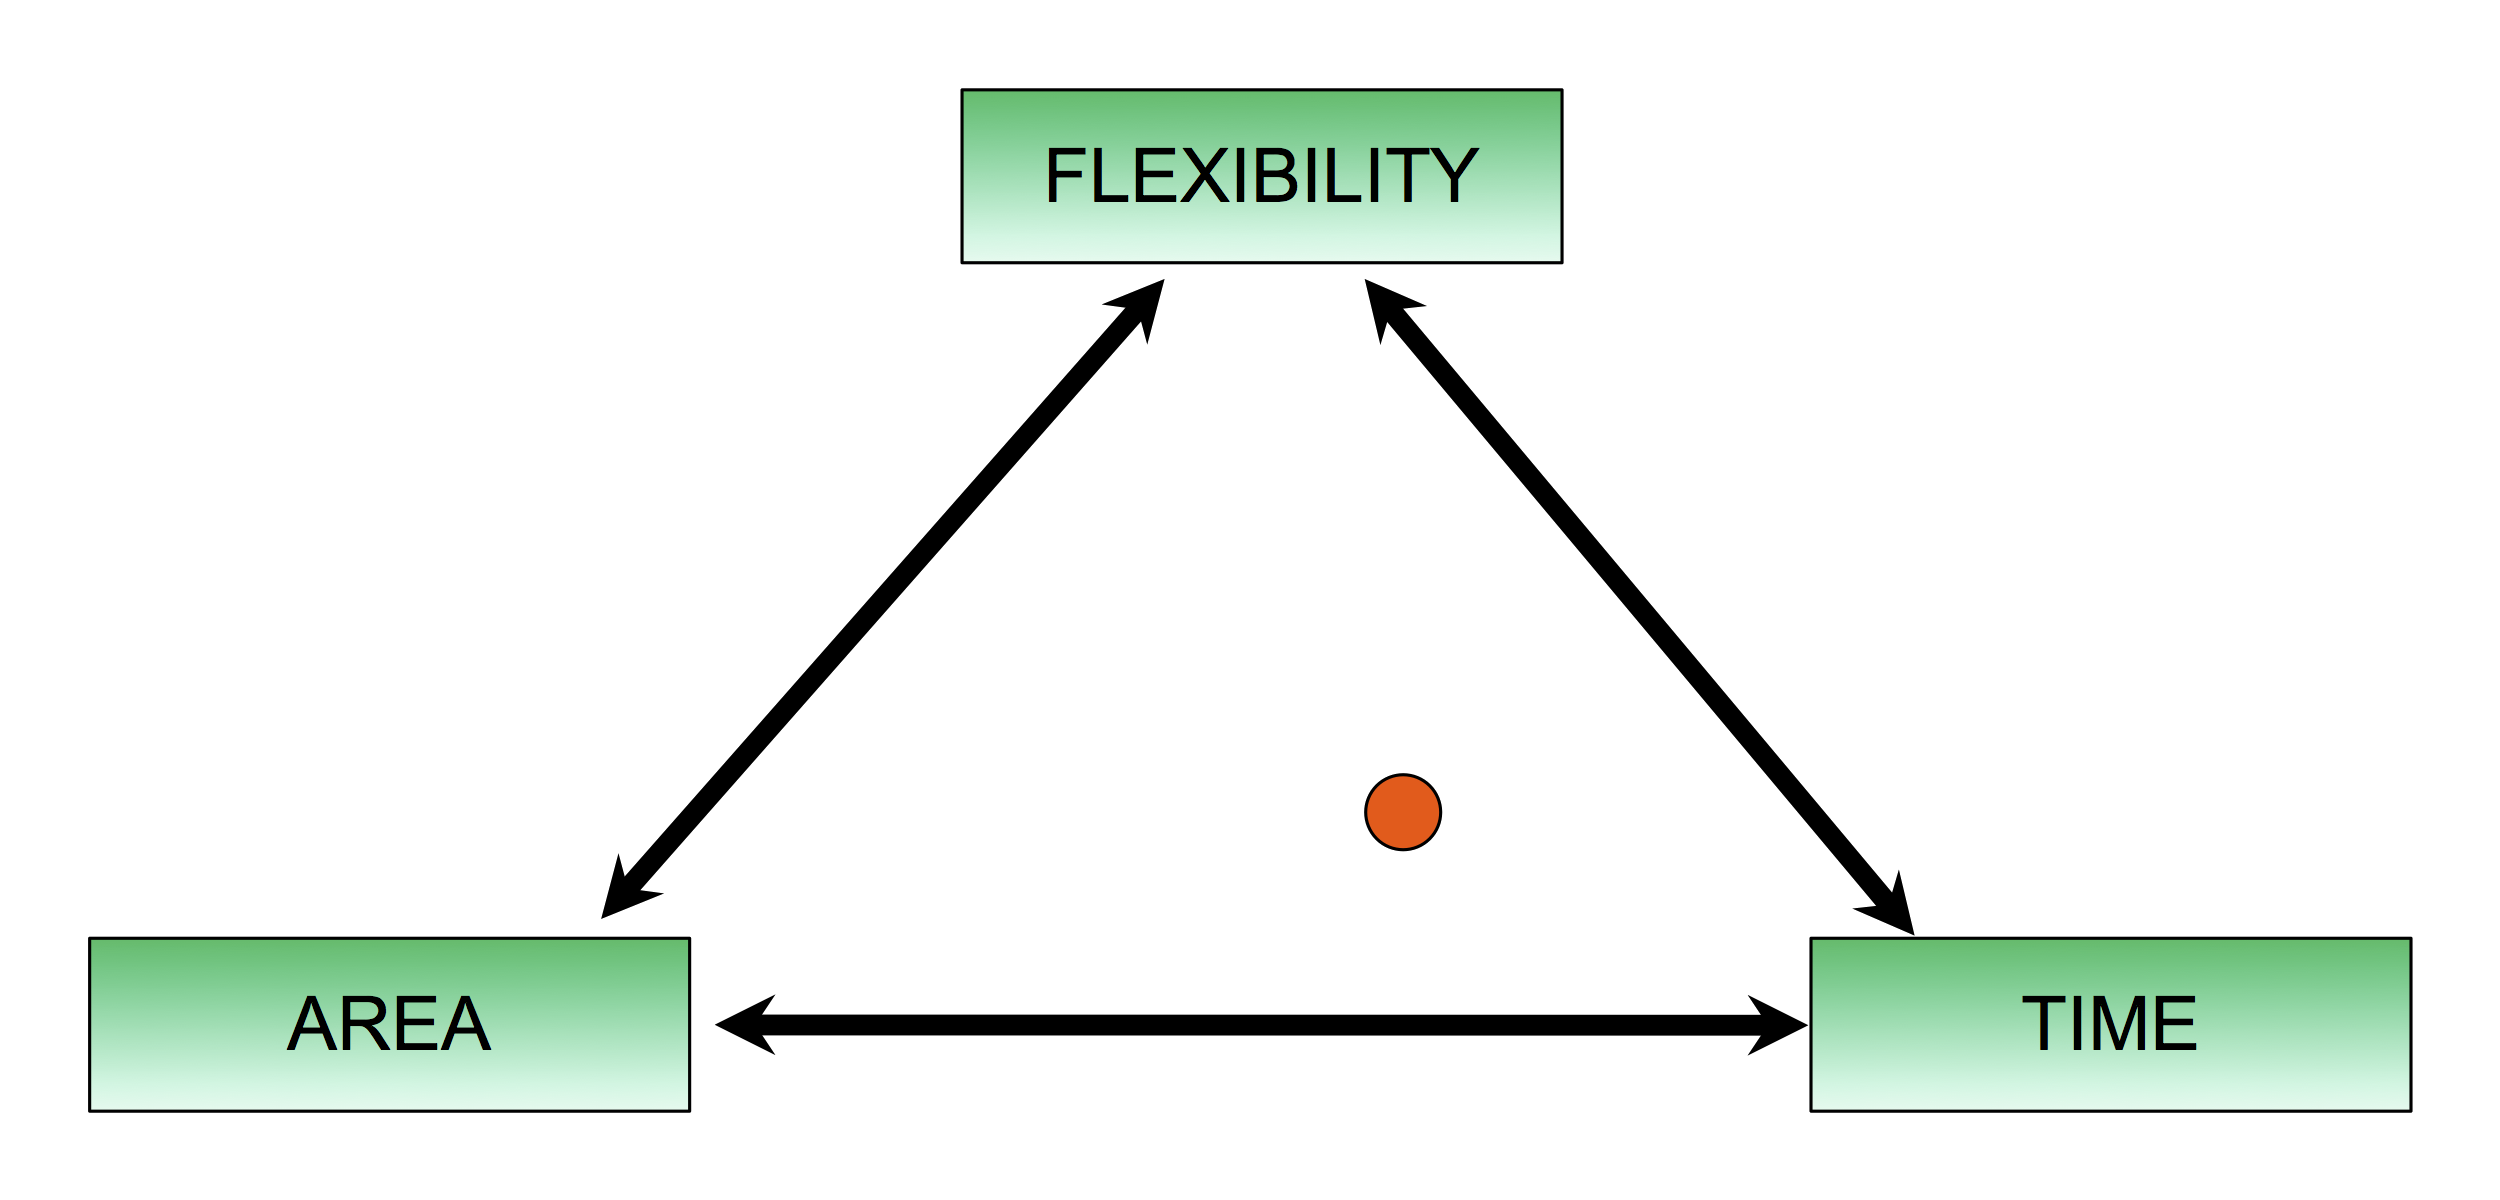
\includegraphics[width=0.5\linewidth]{situation_winter.png}}
	\caption{Situation --- Winter}
	\label{fig:situation_winter}
\end{figure}

\section{Overall Architecture}

Because a complete hardwire implementation was not necessarily faster, when rebuilding the project I decided to rely more on the microprocessor for the exponentiation. Additionally, the coprocessor's size had to be reduced considerably while increasing its maximum frequency. I also wanted to achieve this while keeping the cycle count the same or lower.\\

\begin{figure}[H]
	\center{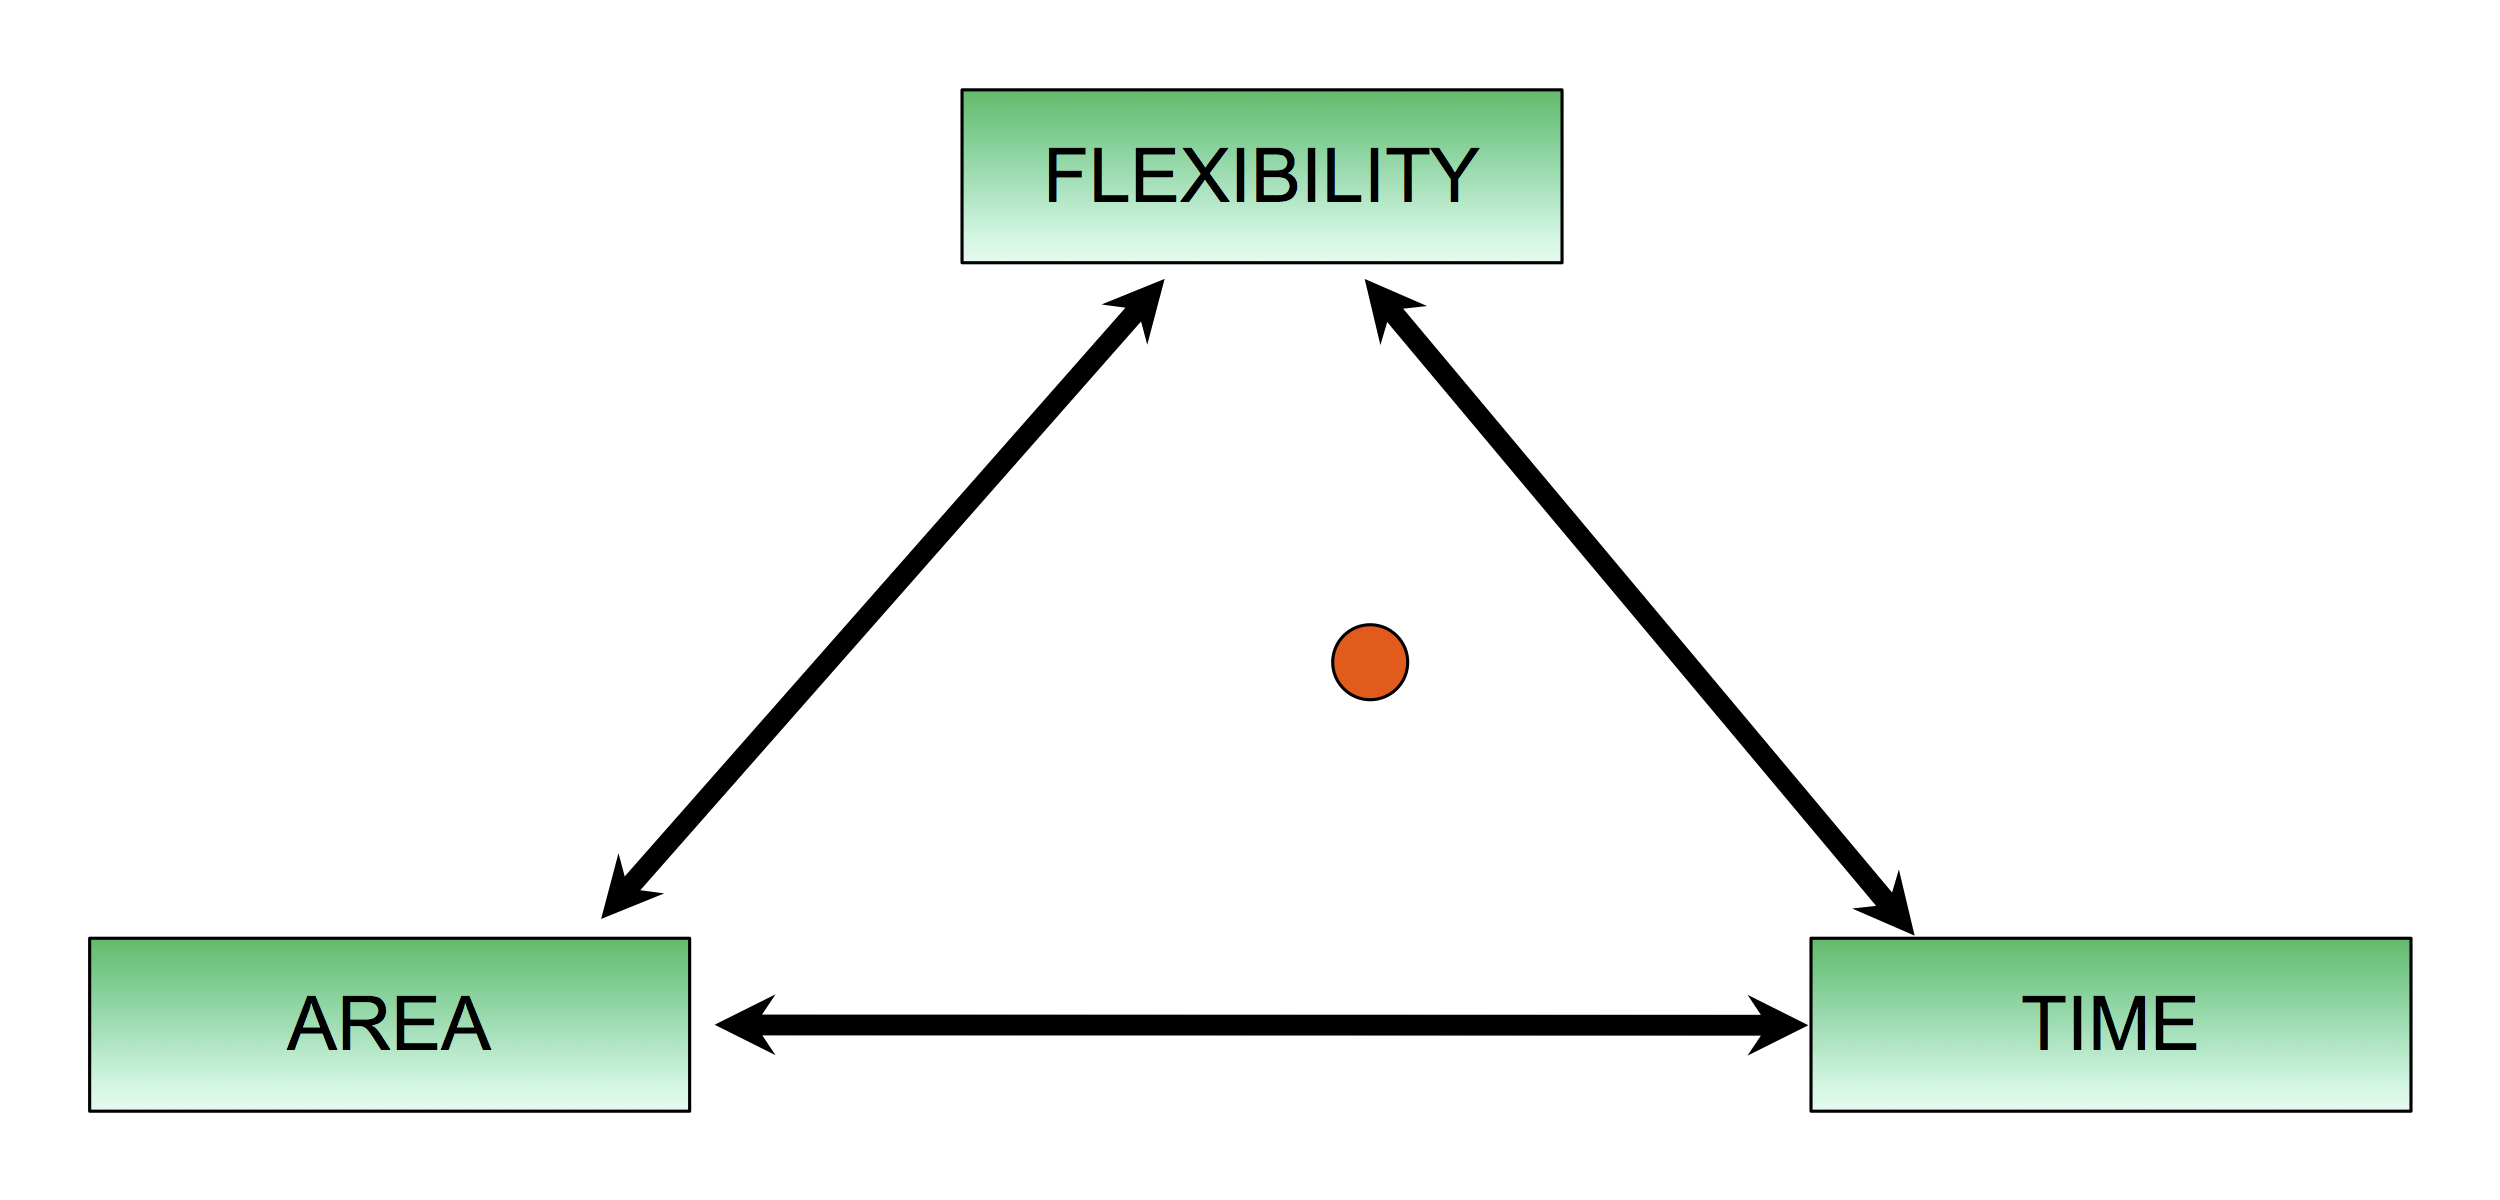
\includegraphics[width=0.5\linewidth]{situation.png}}
	\caption{Situation}
	\label{fig:situation_winter}
\end{figure}

Doing more in software resulted in greater flexibility during the development process. It made it easier to optimize  code and  future, more complex algorithmic optimizations possible (which may be supported by additional hardware features in the coprocessor).

Starting from the existing decoder and Montgomery multiplier from the winter submissions, I built a hardware Montgomery multiplier that was fully memory-mapped. The different pins ($P1$-$P4$) were again used for the communication between the microprocessor and coprocessor. To reduce the overhead of copying data, instructions were introduced to write the multiplication parameters either from memory or from the result register.

\section{HW/SW Boundaries}

\section{HW/SW Interface}

\section{Performance Metrics}

\subsection{Clock Cycles}

\subsection{Area}

\section{Synthesis Results}

\section{Test Strategy}

\section{Further Optimizations}

\end{document}